

\begin{figure}[H]
\centering


	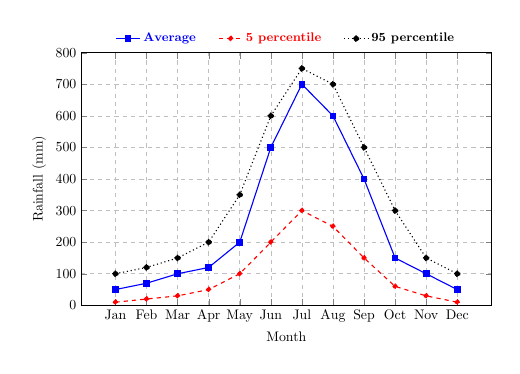
\begin{tikzpicture}[scale = 0.5]
    \begin{axis}[
        width=12cm, height=8cm,
        xlabel={Month},
        ylabel={Rainfall (mm)},
        xtick=data,
        xticklabels={Jan, Feb, Mar, Apr, May, Jun, Jul, Aug, Sep, Oct, Nov, Dec},
        ymin=0, ymax=800,
        ytick={0,100,200,300,400,500,600,700,800},
        legend style={
            at={(0.5,1.1)}, 
            anchor=north, 
            legend columns=3, 
            draw=none, 
            font=\small,
            /tikz/every even column/.append style={column sep=0.5cm}
        },
        legend cell align={left},
        ymajorgrids=true,
        xmajorgrids=true,
        grid style=dashed,
    ]
    
    % Average rainfall data
    \addplot[
        color=blue,
        mark=square*,
        thick
    ]
    coordinates {
        (1,50) (2,70) (3,100) (4,120) (5,200) (6,500) (7,700) (8,600) (9,400) (10,150) (11,100) (12,50)
    };
    \addlegendentry{\textcolor{blue}{\textbf{Average}}}
    
    % 5 percentile rainfall data
    \addplot[
        color=red,
        mark=diamond*,
        dashed,
        thick
    ]
    coordinates {
        (1,10) (2,20) (3,30) (4,50) (5,100) (6,200) (7,300) (8,250) (9,150) (10,60) (11,30) (12,10)
    };
    \addlegendentry{\textcolor{red}{\textbf{5 percentile}}}
    
    % 95 percentile rainfall data
    \addplot[
        color=black,
        mark=*,
        dotted,
        thick
    ]
    coordinates {
        (1,100) (2,120) (3,150) (4,200) (5,350) (6,600) (7,750) (8,700) (9,500) (10,300) (11,150) (12,100)
    };
    \addlegendentry{\textcolor{black}{\textbf{95 percentile}}}
    
    \end{axis}
\end{tikzpicture}
\end{figure}

